\subsection{Mean squared error (MSE)}
Ein naiver Ansatz zwei Bilder auf visuelle Ähnlichkeit zu bewerten, wäre es
iterativ alle Pixelintensitäten miteinander zu vergleichen. Als Werkzeug zum
Vergleich dient hierbei die mittlere quadratische Abweichung
\parencite{mse-overview}. Je niedriger der Abstand, desto mehr stimmen die
Bilder miteinander überein. Obwohl dieses Verfahren eine schnelle Performance
aufweist, ist es nur für Fälle geeignet, bei denen das Referenz- und das 
Suchbild fast identisch sind. Bereits kleine Helligkeitsänderungen, bei
gleichbleibendem Inhalt, ergeben nach Berechnung, des euklidischen Abstands,
eine hohe mittlere quadratische Abweichung (siehe Abbildung
\ref{fig:mse-naive}). \parencite{mse-naive-approach}

\begin{figure}[H]
    \centering
    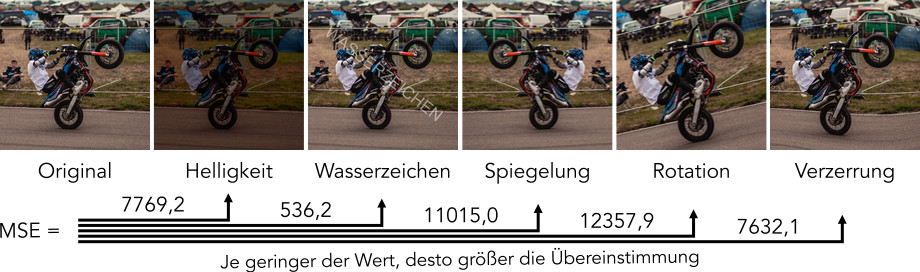
\includegraphics[width=\textwidth]{mse-naive-approach}
    \caption{MSE: Anwendung an verschiedenen Testbildern}
    \label{fig:mse-naive}
    \bildquelle{Eigene Darstellung}
\end{figure}